\section*{Problema 2}
\textbf{Escribe un programa que implemente la estructura de datos Stack usando un arreglo de enteros. Se puede asumir que la capacidad máxima del Stack es de 10 enteros.}

El stack es una estructura de datos que permite almacenar información. El modo de acceso a los datos es de tipo ultimo en entrar, primero en salir (LIFO por sus siglas en inglés). El manejo de los datos se maneja con dos operaciones llamadas \textit{push} y \textit{pop}, las cuales ingresan y retiran información respectivamente del stack. En la figura \ref{fig:stack} se representa visualmente el stack junto a sus operaciones.

\begin{figure}[H]
    \centering
    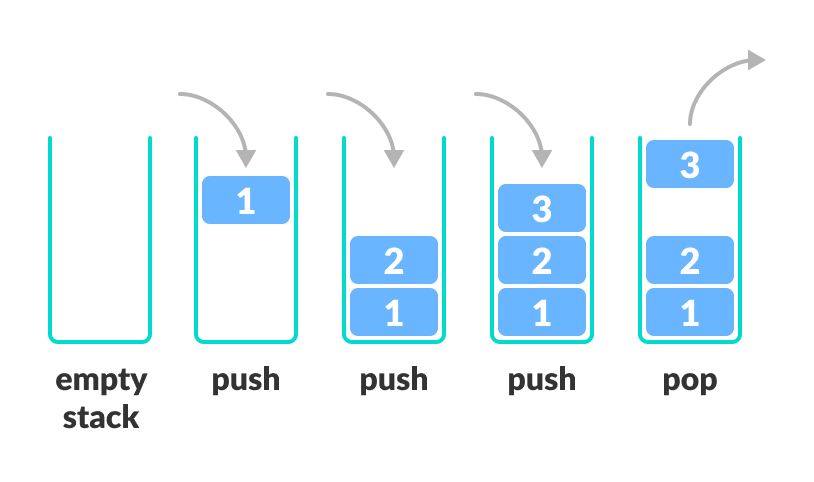
\includegraphics[width=10cm]{Graphics/stack.png}
    \caption{Representación de la estructura de datos stack. Imagen obtenida de \href{https://cdn.programiz.com/sites/tutorial2program/files/stack.png}{Programiz}.}
    \label{fig:stack}
\end{figure}

El pograma realiza las siguentes acciones:

\begin{lstlisting}
    Create stack
    Push(2)
    Push(3)
    Push(4)
    Push(5)
    Push(6)
    Pop
    Pop
    Pop
    Push(4)
    Push(5)
\end{lstlisting}

El output del programa es el siguiente:
\begin{lstlisting}[language=bash]
    --------------------------
    Push number 2:
    2 |
    --------------------------
    Push number 3:
    2 | 3 |
    --------------------------
    Push number 4:
    2 | 3 | 4 |
    --------------------------
    Push number 5:
    2 | 3 | 4 | 5 |
    --------------------------
    Push number 6:
    2 | 3 | 4 | 5 | 6 |
    --------------------------
    pop:
    2 | 3 | 4 | 5 |
    --------------------------
    pop:
    2 | 3 | 4 |
    --------------------------
    pop:
    2 | 3 |
    --------------------------
    Push number 4:
    2 | 3 | 4 |
    --------------------------
    Push number 5:
    2 | 3 | 4 | 5 |
\end{lstlisting}

El programa se encuentra en la carpeta \textcolor{citecolor}{Problema\_2}. Para compilarlo se uso el siguiente comando:

\begin{lstlisting}[language=bash]
    gcc -Wall -Wextra -Werror -pedantic -ansi -o main.out main.c -std=c11
\end{lstlisting}